\documentclass[titlepage,12pt,a4paper,times]{book}

\usepackage[utf8]{inputenc}
\usepackage[portuguese]{babel}
% substituir linha anterior por 
% \usepackage[english]{babel} 
% se o relatório for escrito na língua inglesa.
\usepackage[T1]{fontenc}
\usepackage{makeidx}
\usepackage{xspace}
\usepackage{graphicx,color,times}
\usepackage{fancyhdr}
% \usepackage{pxfonts}
% \usepackage{times}
% \usepackage{mathptm}
% \usepackage{amssymb}
% \usepackage{amsfonts}
\usepackage{amsmath}
\usepackage{latexsym}
\usepackage[printonlyused]{acronym}
\usepackage{float}
\usepackage{listings}
\usepackage{tocbibind}
\usepackage{wrapfig}
\usepackage{natbib}
\usepackage{hyperref}
% \usepackage{glossaries}
% \makeglossaries

\renewcommand{\ttdefault}{phv}

\pagestyle{fancy}
\renewcommand{\chaptermark}[1]{\markboth{#1}{}}
\renewcommand{\sectionmark}[1]{\markright{\thesection\ #1}}
\fancyhf{} \fancyhead[LE,RO]{\bfseries\thepage}
\fancyhead[LO]{\bfseries\rightmark}
\fancyhead[RE]{\bfseries\leftmark}
\renewcommand{\headrulewidth}{0.5pt}
\renewcommand{\footrulewidth}{0pt}
\addtolength{\headheight}{0.5pt}
\setlength{\marginparsep}{0cm}
\setlength{\marginparwidth}{0cm}
\setlength{\marginparpush}{0cm}
\addtolength{\hoffset}{-1.0cm}
\addtolength{\oddsidemargin}{\evensidemargin}
\addtolength{\oddsidemargin}{0.5cm}
\addtolength{\evensidemargin}{-0.5cm}


% NEW COLORS
\definecolor{dark}{gray}{0.25}
\definecolor{lgray}{gray}{0.9}
\definecolor{dkblue}{rgb}{0,0.13,0.4}
\definecolor{dkgreen}{rgb}{0,0.6,0}
\definecolor{gray}{rgb}{0.5,0.5,0.5}
\definecolor{mauve}{rgb}{0.58,0,0.82}

\lstset{ %
  language=C,                    basicstyle=\footnotesize,
  numbers=none,                  numberstyle=\tiny\color{gray}, 
  stepnumber=1,                  numbersep=5pt,
  backgroundcolor=\color{white}, showspaces=false,
  showstringspaces=false,        showtabs=false,
  frame=single,                  rulecolor=\color{black},
  tabsize=2,                     captionpos=b,
  breaklines=true,               breakatwhitespace=false,
  title=\lstname,                keywordstyle=\color{blue},
  commentstyle=\color{dkgreen},  stringstyle=\color{mauve},
  escapeinside={\%*}{*)},        morekeywords={*},
  belowskip=0cm
}

\renewcommand{\lstlistingname}{Excerto de Código}
\renewcommand{\lstlistlistingname}{Lista de Excertos de Código}% 

\begin{document}


\thispagestyle{empty}
\setcounter{page}{-1}

\begin{center}
\begin{Huge}
\textbf{Universidade da Beira Interior}
\end{Huge}
\end{center}

\begin{center}
\begin{Huge}
Departamento de Informática
\end{Huge}
\end{center}

\vspace{0,07cm}
\begin{figure}[!htb]
\centering

\includegraphics[width=191pt]{ubi-fe-di.png}
\end{figure}

\vspace{0.5cm}
\begin{center}
\begin{Large}
\textbf{N\textordmasculine{} 93 - 2020: \emph{Sistema de detecção e tracking de objectos em movimentocom base em análise de imagem}}
\end{Large}
\end{center}


\vspace{0.5cm}
\begin{center}
\begin{normalsize}
\begin{large}
Elaborado por:
\end{large}
\end{normalsize}
\end{center}

\vspace{0.2cm}
\begin{center}
\begin{large}
\textbf{David Miguel Martins Pires}
\end{large}
\end{center}

\vspace{0,5cm}
\begin{center}
\begin{normalsize}
\begin{large}
Orientador:
\end{large}
\end{normalsize}
\end{center}

\vspace{0.2cm}
\begin{center}
\begin{large}
\textbf{Professor Doutor Pedro Domingues de Almeida}
\end{large}
\end{center}



\vspace{0.5cm}
\begin{center}
\begin{normalsize}
26 de Fevereiro de 2020
\end{normalsize}
\end{center}


\clearpage{\thispagestyle{empty}\cleardoublepage}

\frontmatter

\chapter*{Agradecimentos}
\label{chap:ack}

A conclusão deste trabalho, bem como da grande maior parte da minha vida académica não seria possível sem a ajuda de ... 

\clearpage{\thispagestyle{empty}\cleardoublepage}


\tableofcontents

\clearpage{\thispagestyle{empty}\cleardoublepage}

\listoffigures

% Se não existirem tabelas, comentar as seguintes linhas
\clearpage{\thispagestyle{empty}\cleardoublepage}
\listoftables

% Se existirem trechos de código, descomentar as seguintes linhas
% \clearpage{\thispagestyle{empty}\cleardoublepage}
% \lstlistoflistings

\clearpage{\thispagestyle{empty}\cleardoublepage}
\chapter*{Acrónimos}
\label{chap:acro}

% #   ATENÇÃO
% A lista de acrónimods deve ser ordenada alfanumericamente.
% Estrangeirismos devem ser realçados em itálico.
% Se o relatório for escrito em Inglês, uma palavra portuguesa é um estrangeirismo.

% O maior acrónimo deve ser colocado neste ponto
%               vvv
\begin{acronym}[GOTURN]
  \acro{2D}{\emph{2 Dimenções}}
  \acro{3D}{\emph{3 Dimenções}}
  \acro{AI}{\emph{Artificial Intelligence}}
  \acro{AP}{\emph{Average precision}}
  \acro{API}{\emph{Application Programming Interface}}
  \acro{CNN}{\emph{Convolutional Neural Network}}
  \acro{GOTURN}{\emph{Generic Object Tracking Using Regression Networks}}
  \acro{IA}{\emph{Inteligência Artificial}}
  \acro{ID}{\emph{Identification (Identificação)}}
  \acro{IoU}{\emph{Intersection over union}}
  \acro{KCF}{\emph{Kernelized Correlation Filters}}
  \acro{LSTM}{\emph{Long Short Term Memory}}
  \acro{mAP}{\emph{mean Average precision}}
  \acro{MDNet}{\emph{Multi-Domain Convolutional Neural Network Tracker}}
  \acro{OpenCV}{\emph{Open Source Computer Vision Library}}
  \acro{R-CNN}{\emph{Region-based Convolutional Neural Network}}
  \acro{R-FCN}{\emph{Region-based Fully Convolutional Network}}
  \acro{RoI}{\emph{Region of Interest}}
  \acro{ROLO}{\emph{Recurrent YOLO}}
  \acro{RPN}{\emph{Region Proposal Network}}
  \acro{SSD}{\emph{Single Shot Detector}}
  \acro{SVM}{\emph{Support Vector Machine}}
  \acro{YOLO}{\emph{You Only Live Once}}
\end{acronym}


%% !!!!!! LER PRIMEIRAS LINHAS ANTES DE VERSÃO FINAL !!!!!!!!!




% \clearpage{\pagestyle{empty}\cleardoublepage}
% \chapter*{Glossário}
\makeglossaries

\newglossaryentry{.NET Framework}
{
  name={.NET Framework},
  description={É uma plataforma para desenvolvimento e funcionamento de aplicações desenvolvida pela Microsoft.}
}

\newglossaryentry{ASP.NET}
{
  name={ASP .Net},
  description={É uma plataforma da Microsoft para o desenvolvimento de aplicações Web e é o sucessor da tecnologia ASP.}
}

\newglossaryentry{CS}
{
  name={C\#},
  description={Lê-se \textit{C Sharp} e é uma linguagem de programação orientada a objectos, desenvolvida pela Microsoft, inicialmente para a plataforma .NET. O C\# é inspirado na junção entre as linguagens C++ e Java.}
}


\newglossaryentry{Java}
{
  name={JAVA},
  description={É uma linguagem de programação orientada a objectos, desenvolvida pela Sun Microsystems na década de 90. Hoje pertence à empresa Oracle.}
}


\newglossaryentry{OpenDMTP}
{
  name={OpenDMTP},
  description={\textit{Open Device Monitoring and Tracking Protocol} é um protocolo e uma \textit{framework} abertos que permite a comunicação bidireccional entre servidores e clientes através da internet.}
}


\newglossaryentry{OpenGTS}
{
  name={Open GTS},
  description={É o primeiro projecto \textit{Open Source} \textit{Web-Based} para controlo de frotas por GPS.}
}


\newglossaryentry{VS2010}
{
  name={Visual Studio 2010},
  description={\textit{Microsoft Visual Studio 2010} é um sistema de desenvolvimento desenvolvido pela Microsoft e é dedicado ao Framework .NET, que contem um conjunto de ferramentas de desenvolvimento projectadas para auxiliar os programadores a enfrentarem desafios complexos.}
}


\newglossaryentry{WebS}
{
	name={Web Service},
	description={Web services são aplicações modulares auto-descritas e auto-contidas, que permitem a integração de sistemas e a comunicação entre aplicações de diferentes tipos.}
}


\newglossaryentry{WebBased}
{
	name={Web Based},
	description={Aplicação desenvolvida para a Web.}
}

\newglossaryentry{Roaming}
{
	name={Roaming},
	description={Define a possibilidade de um utilizador de uma determinada rede obter rede/conecção fora da área geográfica onde foi registado.}
}


\newglossaryentry{Smartphone}
{
	name={Smartphone},
	description={Smartphone é um telefone móvel que contem muitas das principais tecnologias de comunicação e serviços que existem nos computadores pessoais, como acesso a e-mails, serviços de mensagens instantâneas, internet, GPS, entre outros.}
}

\newglossaryentry{TCPIP}
{
	name={TCP/IP},
	description={É um conjunto de protocolos de comunicação entre computadores ligados rede. O nome TCP/IP surge da união entre dois protocolos: o TCP (Transmission Control Protocol) e o protocolo IP (Internet Protocol).}
}

\newglossaryentry{Firewall}
{
	name={Firewall},
	description={É o nome criado para definir um dispositivo para uma rede de computadores que tem como objectivo criar uma política de segurança num determinado ponto de controlo da rede.}
}

\newglossaryentry{JavaScript}
{
	name={JavaScript},
	description={É uma linguagem de programação baseada na linguagem de programação ECMAScript. Actualmente é a linguagem de programação mais utilizada em \textit{``Client-Side''} nos \textit{browsers}.}
}

\newglossaryentry{Flash}
{
	name={Flash},
	description={Desenvolvido pela Macromedia, o Flash é um software utilizado para criação de animações interactivas que funcionam incorporadas em \textit{Browsers}, \textit{Desktop}, \textit{Smartphones}, \textit{Tablets}, e Televisores.}
}


\newglossaryentry{StoredProcedure}
{
	name={Stored Procedure },
	description={É o nome dado a um conjunto de comandos numa base de dados de forma a simplificar a sua utilização.}
}

\newglossaryentry{SQLS}
{
	name={SQL Server 2008},
	description={É um sistema de gestão de base de dados relacional criado pela Microsoft.}
}

\newglossaryentry{Firm}
{
	name={Firmware},
	description={É o conjunto de instruções operacionais programadas directamente no \textit{hardware} de um equipamento electrónico.}
}

\newglossaryentry{browser}
{
	name={Browser},
	description={É um programa de computador que possibilita aos utilizadores uma interacção com documentos virtuais da Internet, também conhecidos como páginas Web.}
}



\clearpage{\thispagestyle{empty}\cleardoublepage}

\mainmatter
\acresetall
\chapter{Introdução}
\label{chap:intro}

% CADA SECÇÃO DEVE TER UM LABEL
% CADA FIGURA DEVE TER UM LABEL
% CADA TABELA DEVE TER UM LABEL

\section{Enquadramento}
\label{sec:amb}

Sistema de detecção e tracking de objectos em movimentocom base em análise de imagem

- Visão Computacional
- Identificação de objetos em imagem (2D, 3D) ou em um video sobre um ambiente de luz natural.
Desafio para os sistemas de Visão Computacional, sendo que já foram implementadas muitas abordagens para estes sistemas ao longo dos anos.
- O Tranking de objetos é tambem um desafio para estes sistemas de Visão Computacional.

Neste projeto todo o codigo é desenvolvido usando um Raspberry Pi, com capacidades limitadas, o que torna este trabalho ainda um maior defafio ao nivel da Complexidade Computacional.

- Complexidade Computacional 

Usaremos tambem uma camera comum e conectada ao Raspberry Pi para obter as imagens para analisar em tempo real. Usarei uma camera da marca Logitech que tenho em casa, conectada via USB.

Para isto iremos usar irei usar um Raspnerry Pi 4, Modulo B de 4GB RAM que tenho em casa e um cartão de memória de 64 Gb.

\section{Motivação}
\label{sec:mot}

O tema deste projeto é um tema atual e muito importante para as áreas de Visão Computacional e da Robotica. Daí ser uma grande motivação minha na escolha deste trabalho.

O reconhecimento de objetos será sempre uma area imprencindivel e de grande interesse para a robotica. Neste caso iremos reconhecer alguns objetos e rastrealos em um fluxo de video. 
Isto ainda em um ambiente de desenvolvimento com capacidades bastante limitadas, que é o Raspberry Pi, o que torna esta tarefa um desafio. 

Apesar de nós humanos, conseguirmos reconhecer múltiplos objetos em diferentes imagens, e em diferentes disposições em segundos sem qualquer dificuldade. Muitas vezes mesmo Objetos obtruidos por outros objetos. Isto para a Visão Computacional é ainda um desafio, e é muito mais complexo reconhecer um objeto em uma imagem do que pensamos à primeira vista.

- Lab 
- Prof
- Raspberry Pi

----- Old:

A motivação da escolha deste projeto como projeto deve-se ao meu interesse neste tema de projeto. Tenho também muito interesse no aprendizado das ferramentas utilizadas como por exemplo a programação em um dispositivo com capacidades reduzidas, como um \ac{Raspberry}.


\section{Objetivos}
\label{sec:obj}

Como objetivo deste trabalho temos a elaboração de um Sistema de deteção e traking de objetos em movimento com base em análise de imagem. Este sistema deve ser desenvolvido para posteriormente ser usado em um Raspberry Pi, com capacidade de processamento limitada. Devemos também usar uma webcam e ferremntas de programação como Tensorflow, Opencv e Yolo.

\section{Organização do Documento}
\label{sec:organ}
% !POR EXEMPLO!
De modo a refletir o trabalho que foi feito, este documento encontra-se estruturado da seguinte forma:
\begin{enumerate}
\item O primeiro capítulo -- \textbf{Introdução} -- apresenta o projeto, a motivação para a sua escolha, o enquadramento para o mesmo, os seus objetivos e a respetiva organização do documento.
\item O segundo capítulo -- \textbf{Tecnologias Utilizadas} -- descreve os conceitos mais importantes no âmbito deste projeto, bem como as tecnologias utilizadas durante do desenvolvimento da aplicação.
\item ...
\end{enumerate}

% 
\section{Algumas Dicas -- [RETIRAR DA VERSÃO FINAL]}
% ALGUMAS DICAS
Os relatórios de projeto são individuais e preparados em \LaTeX, seguindo o formato disponível na página da unidade curricular. Deve ser prestada especial atenção aos seguintes pontos:
\begin{enumerate}
  \item O relatório deve ter um capítulo Introdução e Conclusões e Trabalho Futuro (ou só Conclusões);
  \item A última secção do primeiro capítulo deve descrever suscintamente a organização do documento;
  \item O relatório pode ser escrito em Língua Portuguesa ou Inglesa;
  \item Todas as imagens ou tabelas devem ter legendas e ser referidas no texto (usando comando \texttt{\textbackslash ref\{\}}).
\end{enumerate}
\clearpage{\thispagestyle{empty}\cleardoublepage}
\chapter{Estado da Arte}
% OU \chapter{Trabalhos Relacionados}
% OU \chapter{Engenharia de Software}
% OU \chapter{Tecnologias e Ferramentas Utilizadas}
\label{chap:estado-da-arte}

\section{Introdução}
\label{chap2:sec:intro}

O reconhecimento e rastreamento de objetos é um dos campos mais atuais da visão computacional.
\newline É possível reconhecer diferentes objetos em uma cena através das suas formas, cor e diferentes características do objeto.
É também possível rastrear um objeto em um fluxo de vídeo através do calculo de distâncias, comparação de formas, e outras características.
\newline Neste capitulo será abordado o estado atual do reconhecimento de objetos e o estado atual do rastreamento de objetos, e diferentes algoritmos que existem para o fazer. Isto com a especial atenção ao meio de desenvolvimento que será um Raspberry Pi, um pequeno computador com capacidades limitadas.
\paragraph{Este capítulo está estruturado da seguinte forma:}
\begin{enumerate}
  \item Secção 2.1 - \textbf{Algoritmos de reconhecimento de objetos} - Esta secção apresenta vários algoritmos estudados sobre a deteção/reconhecimento de objetos e uma breve explicação do seu funcionamento. 
  \item Secção 2.2 - \textbf{Algoritmos de rastreamento de objetos} - Esta secção apresenta vários algoritmos estudados sobre o rastreamento de objetos, e uma breve explicação do seu funcionamento.
  \item Secção 2.3 - \textbf{Conclusões} - Esta secção apresentará uma breve conclusão sobre este capitulo.
\end{enumerate}

\section{Algoritmos de reconhecimento de objetos}
\label{chap2:sec:estadoatual}

\paragraph{}
A deteção de objetos combina as tarefas de localização e classificação de objetos. Corresponde a localizar um objeto em uma imagem e adivinhar que objeto é esse, como vemos na figura \ref{img:classificacaolocalizacao}. Em vez de prevermos a classe de objeto a partir de uma imagem, agora temos de prever a classe e também um rectângulo, chamada caixa delimitadora, contendo esse objeto.

\begin{figure}[h!]
  \centering
  \label{img:classificacaolocalizacao}
  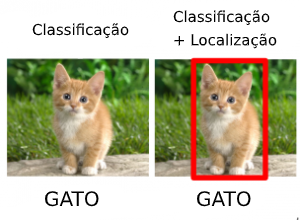
\includegraphics[width=0.5\textwidth]{classificationmorelocalization.png}
  \caption{Ilustração de classificação e localização de um objeto/pessoa em uma imagem.}
\end{figure}

São necessárias 4 variáveis para identificar exclusivamente um retângulo. Portanto, para cada instância do objeto na imagem, preveremos as seguintes variáveis:
\begin{itemize}
    \item nome\_da\_classe
    \item caixa\_delimitadora\_topo\_esquerda\_coordenada\_x
    \item caixa\_delimitadora\_topo\_esquerda\_coordenada\_y
    \item caixa\_delimitadora\_altura
    \item caixa\_delimitadora\_largura
\end{itemize}

Nas subsecções abaixo abordarei alguns algoritmos de deteção de objetos populares. Historicamente, tem havido muitas abordagens para deteção de objetos a partir de Haar cascades, proposta por Viola e Jones em 2001. No entanto, irei focar nos métodos de ponta que usam Redes Neurais e Aprendizagem Profunda.

\paragraph{}
Os detectores de objetos atuais podem ser divididos em duas categorias:
\newline - Redes que separam as tarefas de determinar a localização dos objetos e sua classificação, onde Faster \ac{R-CNN} é uma das mais famosas.
\newline - Redes que prevêem caixas delimitadoras e classificações de classes de uma só vez, onde \ac{YOLO} e \ac{SSD} são famosas arquiteturas.

\subsection{Overfeat}
\label{chap2:subsec:overfeat}

\paragraph{}
A primeira rede neural profunda para deteção de objetos foi \textbf{Overfeat}. Eles introduziram uma abordagem de janela deslizante de várias proporções, como mostra na figura \ref{img:janeladeslizante}, e usando uma \ac{CNN}, mostraram que a deteção de objetos também melhorou a classificação de imagens.

\begin{figure}[h!]
  \label{img:janeladeslizante}
  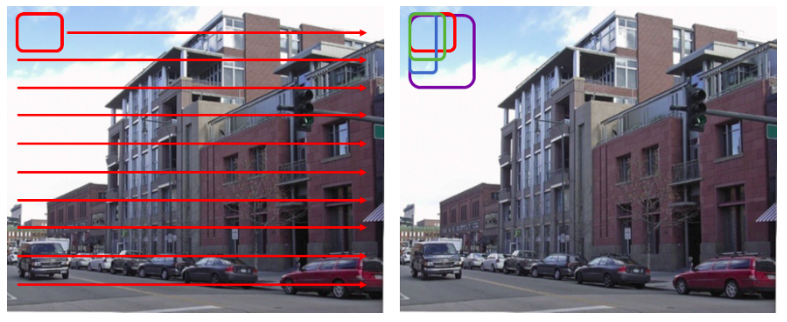
\includegraphics[width=1\textwidth]{janeladeslizante.png}
  \caption{Ilustração de uma janela deslizante (direita) com diferentes proporções (direita).}
\end{figure}


\paragraph{}
\textbf{CNN} é uma rede neural que consiste em várias camadas diferentes, como a camada de entrada (input), pelo menos uma camada escondida e uma camada de saída (output). Esta é usada para reconhecer padrões como pontas, vertical/horizontal, formas, cores e texturas.

\subsection{R-CNN}
\label{chap2:subsec:rcnn}

O modelo anterior foi logo seguindo pelo \textbf{\ac{R-CNN}}:  Regiões com características \ac{CNN}. As \ac{CNN}s são demasiado lentas e dispendiosas, por isso é impossível correr uma \ac{CNN} em tantos caminhos gerados por um detector de janela deslizante. Então a \ac{R-CNN} resolve este problema usando um algoritmo de propostas de objetos chamado de \textbf{Pesquisa seletiva} que reduz o numero de caixas delimitadoras que são alimentadas no classificador para fechar em 2000 propostas de região. A Pesquisa seletiva usa dicas locais como textura, intensidade, cor e/ou a medida de incidências, etc, para gerar todas as propostas de localização do objeto. Cada região é alimentada em uma \ac{CNN}, que produziu um vetor de característica de grande dimensão. Este vetor é depois usado para a classificação final e regressão da caixa delimitadora, como mostra na figura \ref{img:rcnn}.


\begin{figure}[h!]
  \label{img:rcnn}
  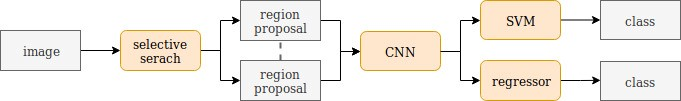
\includegraphics[width=1\textwidth]{rcnn.jpeg}
  \caption{A arquitetura padrão de uma rede \ac{R-CNN} consiste em um método de proporção regional. A classificação final é feita com uma \ac{SVM} e uma regressão.}
\end{figure}

\textbf{\ac{SVM}} é um conjunto de métodos de aprendizado supervisionado que analisam os dados e reconhecem padrões, usando classificação e análise de regressão.

\paragraph{}
Então, existem 3 importantes etapas da \ac{R-CNN}:

\begin{enumerate}
    \item Realizar pesquisa seletiva para gerar prováveis objetos.
    \item Alimentar esses caminhos em uma \ac{CNN}, seguidos de uma \ac{SVM} para prever a classe de cada caminho.
    \item Optimizar os caminhos, treinando as caixas delimitadoras separadamente.
\end{enumerate}

\subsection{Fast R-CNN}
\label{chap2:subsec:fastrcnn}

\paragraph{}
Uma abordagem mais sofisticada, o \textbf{Fast \ac{R-CNN}} também gera proporções regionais com pesquisa seletiva, mas alimenta a imagem inteira através de uma \ac{CNN}.
Ela superou o desempenho da rede Overfeat por uma grande margem, mas ainda assim é muito lenta, porque a geração proposicional usando pesquisa seletiva é muito demorada, tal como a necessidade de alimentar cada proposta através de uma \ac{CNN}. As proporções regionais são agrupadas directamente em um mapa característico por \ac{RoI} pooling. Os vetores característicos agrupados são alimentados em uma rede totalmente conectada para classificação e regressão, como retratado na figura \ref{img:fastrcnn}. Similar ao \ac{R-CNN}, o Fast \ac{R-CNN} gera as proporções regionais usando pesquisa seletiva.

\paragraph{}
\textbf{\ac{RoI} pooling}, ou agrupamento da Região de Interesse é o processo de converter uma região de interesse da imagem original em uma imagem de tamanho fixo para que se possa passar à próxima etapa de deteção do objeto.

\begin{figure}[h!]
  \label{img:fastrcnn}
  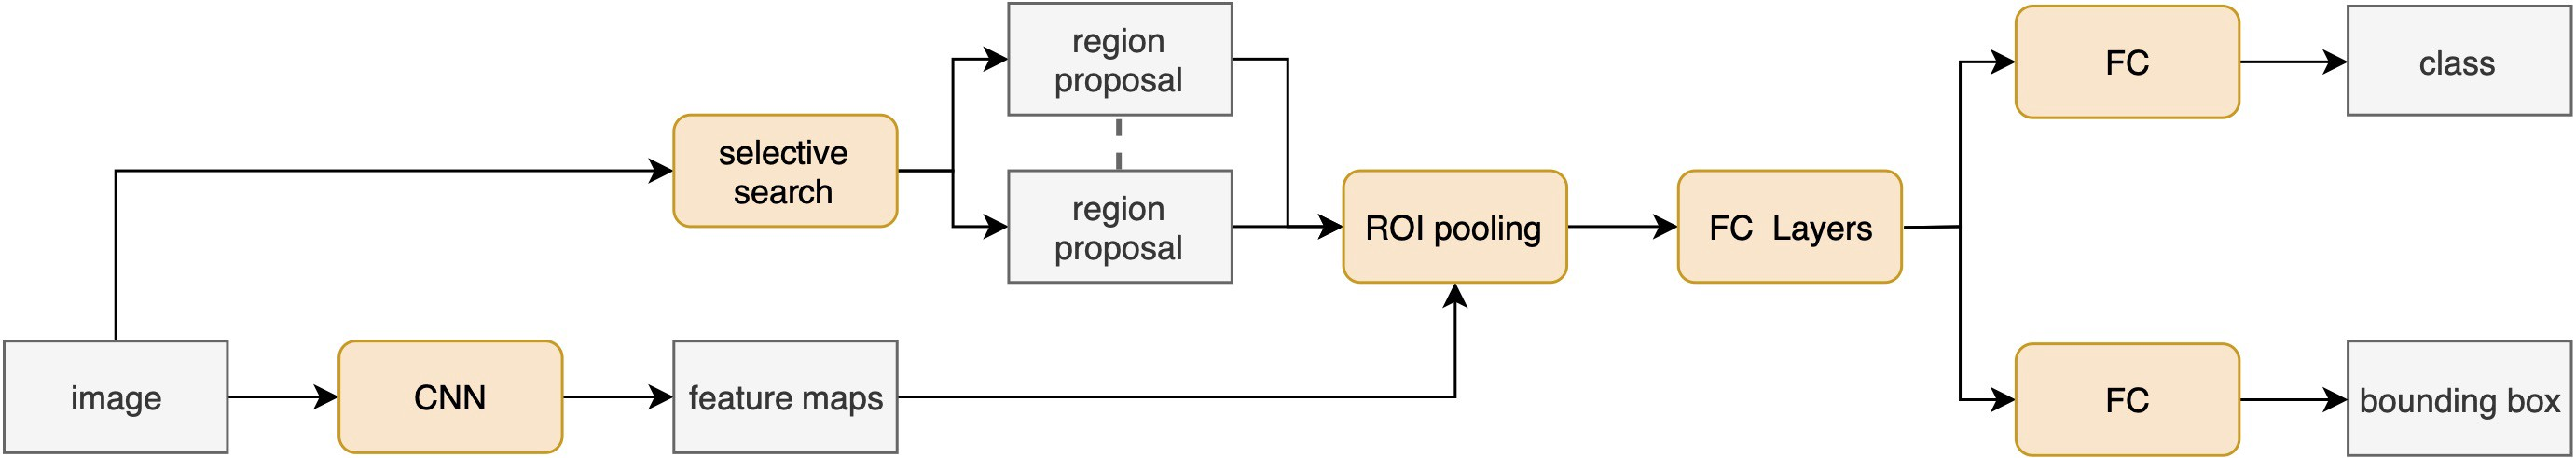
\includegraphics[width=1\textwidth]{fastrcnn.jpeg}
  \caption{A arquitetura padrão da rede Fast-\ac{R-CNN}. A proporção regional é gerada usando pesquisa seletiva, mas agrupada diretamente no mapa de características, seguida de várias camadas FC para a classificação final e regressão da caixa delimitadora.}
\end{figure}

\subsection{Faster R-CNN}
\label{chap2:subsec:fasterrcnn}

\paragraph{}
A parte mais lenta da arquitetura Fast \ac{R-CNN} é a pesquisa selectiva e as caixas de borda. Então a arquitetura \textbf{Faster \ac{R-CNN}} substitui a pesquisa seletiva por uma pequena rede convolucional chamada rede de propostas por região (\ac{RPN}) para gerar regiões de interesse.
\newline Para lidar com as variâncias nas proporções e escala dos objetos, Faster \ac{R-CNN} introduz a ideia de \textbf{caixas âncora}. Em cada localização, o documento original usa 3 tipos de caixas âncora para as escalas 128x128, 256x256 e 512x512. Da mesma forma, para as proporções de 1:1, 1:2 e 2:1. Portanto, em cada local, temos 9 caixas nas quais a \ac{RPN} prevê a probabilidade de ser segundo plano ou primeiro plano. Aplicamos a regressão da caixa delimitadora para melhorar as caixas âncora em cada local. Portanto, a \ac{RPN} fornece-nos caixas delimitadoras de vários tamanhos com as probabilidades correspondentes de cada classe.
A rede restante é semelhante à arquitetura Fast \ac{R-CNN}.

\begin{figure}[h!]
  \label{img:fasterrcnn}
  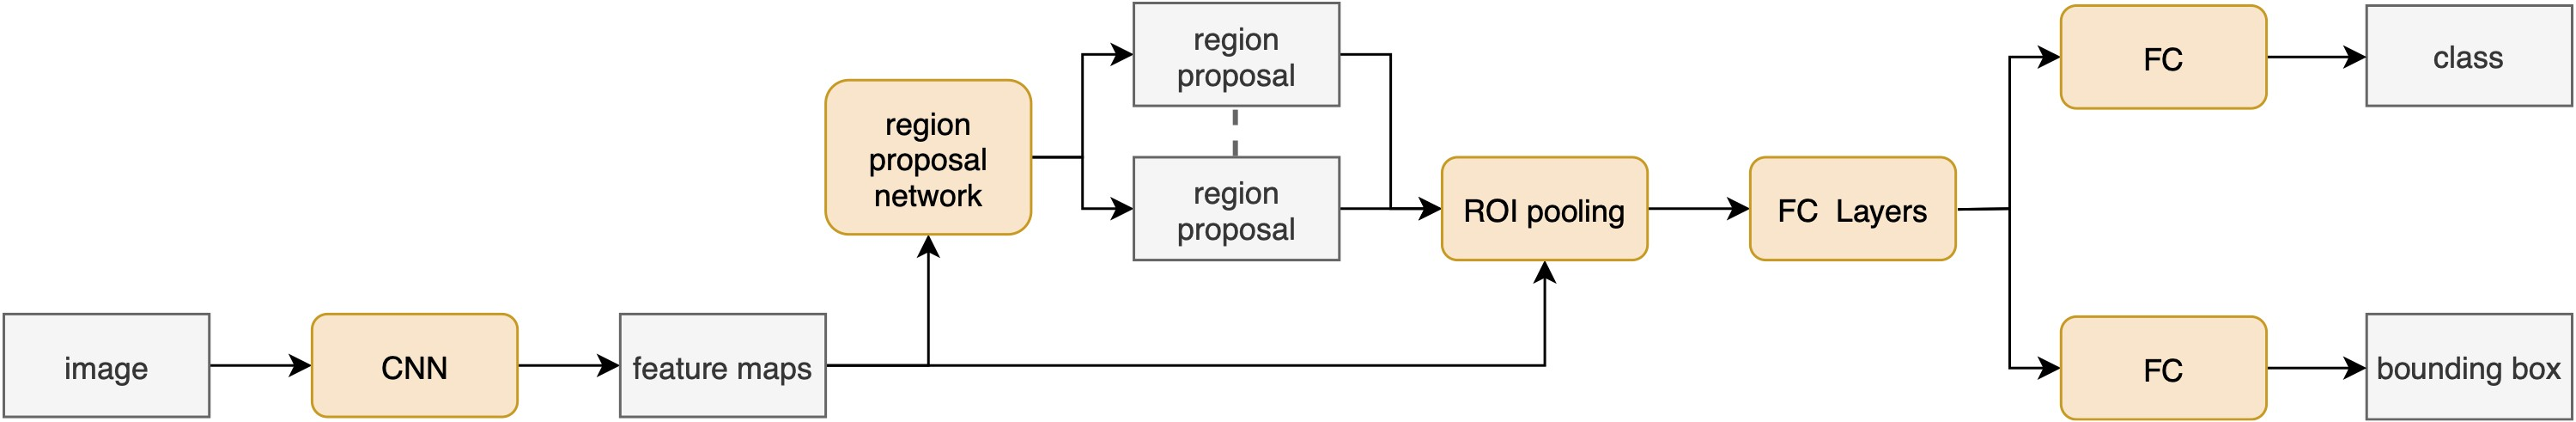
\includegraphics[width=1\textwidth]{fasterrcnn.jpeg}
  \caption{A arquitetura padrão da rede Faster-\ac{R-CNN}, onde a proposta por região é gerada usando uma \ac{RPN}, que trabalha directamente com o mapa de características. As ultimas camadas estão totalmente conectadas para classificação e regressão das caixas delimitadoras.}
\end{figure}

\subsection{YOLO}
\label{chap2:subsec:yolo}

O design das redes de deteção de objetos foi revolucionado pela rede \textbf{\ac{YOLO}}. Este segue uma abordagem completamente diferente dos modelos mencionados e é capaz de prever classificações de classes e caixas delimitadoras de uma vez.
\newline Este modelo divide a imagem em uma grelha S x S, e cada célula prevê N caixas delimitadoras e confiança. A confiança reflete a precisão da caixa delimitadora e se a caixa delimitadora realmente contem o objeto (independentemente da classe). \ac{YOLO} também prevê a pontuação da classificação para cada caixa de cada classe de treinamento. Você pode combinar as duas classes para calcular a probabilidade de cada classe estar presente em uma caixa prevista.

Portanto, são previstas S x S x N caixas. No entanto, muitas dessas caixas tem pontuações baixas de confiança e, se definirmos um limite, digamos que a 30\% de confiança, podemos remover a maioria deles, como mostrado no exemplo \ref{img:yolo}.

\begin{figure}[h!]
  \label{img:yolo}
  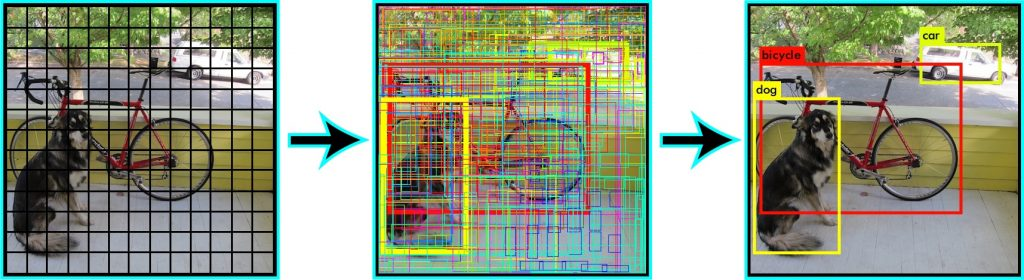
\includegraphics[width=1\textwidth]{yolo.jpg}
  \caption{Exemplo do funcionamento da arquitetura \ac{YOLO}.}
\end{figure}

Os autores libertaram mais três versões, YOLO9000, YOLOv2 e YOLOv3, onde o primeiro é capaz de prever até 9000 categorias, o segundo é capaz de processar imagens maiores e o terceiro é mais preciso. 

\subsection{SSD}
\label{chap2:subsec:ssd}

Outra rede que prevê classes e caixas delimitadoras de uma vez é a \textbf{\ac{SSD}}. Esta executa uma rede convolucional em uma imagem apenas de entrada e calcula um mapa de recursos. Aqui executamos um pequeno núcleo convolucional de tamanho 3 x 3 neste mapa de recursos para prever as caixas delimitadoras e a probabilidade de classificação.
\newline A rede \ac{SSD} também usa caixas âncora em várias proporções semelhantes ao Faster \ac{R-CNN} e aprende o deslocamento em vez de aprender a caixa. Para lidar com a escala, a \ac{SSD} prevê caixas delimitadoras após várias camadas convolucionais. Como cada camada convolucional opera em uma escala diferente, ela é capaz de detectar objetos de várias escalas.

É comparável com o \ac{YOLO}, mas esta usa várias proporções por célula da grelha e mais camadas convolucionais para melhorar a precisão.


% https://towardsdatascience.com/understanding-object-detection-9ba089154df8
% https://cv-tricks.com/object-detection/faster-r-cnn-yolo-ssd/
% https://medium.com/analytics-vidhya/beginners-guide-to-object-detection-algorithms-6620fb31c375

\section{Algoritmos de rastreamento de objetos}
\label{chap2:subsec:algoritmosrastreamento}

\paragraph{}
O rastreamento de objetos é o processo de localizar objetos em movimento ao longo do tempo em vídeo. 
Este é um problema antigo e difícil da visão computacional. Existem várias técnicas e algoritmos que tentam resolver esse problema de várias maneiras diferentes. No entanto, a maioria baseia-se em duas coisas principais:
\begin{itemize}
    \item \textbf{Modelo de movimento}
\newline Um dos principais componentes de uma bom rastreador é a capacidade de entender e modelar o movimento do objeto. Assim, é desenvolvido um modelo de movimento que captura o movimento dinâmico de um objeto. Ele prevê a posição potencial dos objetos nos quadros (frames) seguintes, reduzindo assim o espaço de pesquisa. No entanto, o modelo de movimento por si só pode falhar em cenários em que o movimento é causado por coisas que não estão em um vídeo ou direcção abrupta e mudança de velocidade.
    \item \textbf{Modelo de Aparência Visual}
\newline A maioria dos rastreadores altamente precisos precisa entender a aparência do objeto que eles estão rastreando. Mais importante, eles precisam aprender a discriminar o objeto do plano de fundo. Nos rastreadores de um único objeto, apenas a aparência visual pode ser suficiente para rastrear o objeto através dos quadros, enquanto nos rastreadores de vários objetos, apenas a aparência visual não é suficiente.
\end{itemize}

\paragraph{}
Existem várias características para classificar um rastreador de objetos, como por exemplo:

\begin{itemize}
    \item \textbf{Rastreadores com base na deteção}
    \newline Os quadros de vídeo consecutivos são dados a um detector de objetos pré treinado que fornece uma hipótese de deteção, que por sua vez, é usada para formar trajetórias de rastreamento. Novos objetos são detectados e objetos que desaparecem são finalizados automaticamente. Nesta abordagem, o rastreador é usado para os casos em que a deteção de objetos falha. Em outra abordagem, o detector de objetos é executado para nada N quadros e as previsões restantes são feitas usando o rastreador.
    \item \textbf{Rastreamento sem deteção}
    \newline O rastreamento sem deteção requer inicialização manual de um número fixo de objetos no primeiro quadro. Em seguida, localiza esses objetos nos quadros subsequentes. Esta abordagem não pode lidar com o caso em que novos objetos aparecem nos quadros subsequentes.
    \item \textbf{Acompanhamento de um único objeto}
    \newline Apenas um único objeto é rastreado, mesmo que o ambiente tenha vários objetos. O objeto a ser rastreado é determinado pela inicialização do primeiro quadro.
    \item \textbf{Rastreamento de Objetos múltiplos}
    \newline Todos os objetos presentes são rastreados ao longo do tempo. Se um rastreador baseado em deteção for usado, ele poderá rastrear novos objetos que surjam no meio do vídeo.
    \item \textbf{Rastreamento offline}
    \newline Rastreadores offline são usados quando você precisa rastrear um objeto em um fluxo de gravado. Neste caso, podemos não apenas usar os quadros passados, mas também os futuros quadros para fazer previsões de rastreamento mais precisas.
    \item \textbf{Rastreamento online}
    \newline Rastreadores online são usados onde as previsões estão disponíveis imediatamente, e portanto, estes não podem usar quadros futuros para melhorar os resultados.
    \item \textbf{Rastreamento de aprendizagem online}
    \newline Estes rastreadores geralmente aprendem sobre o objeto a ser rastreado usando o quadro de inicialização e alguns quadros subsequentes. Portanto, esses rastreadores são mais gerais, porque você pode simplesmente desenhar uma caixa delimitadora em torno de um objeto e rastreá-lo.
    \item \textbf{Rastreamento de aprendizagem offline}
    \newline O treinamento destes rastreadores acontece apenas offline. Ao contrário dos rastreadores de aprendizado online, estes rastreadores não aprendem nada durante o tempo de execução. Estes rastreadores aprendem sobre os conceitos completos offline, ou seja, podemos treinar um rastreador para identificar pessoas. Estes rastreadores podem ser usados para rastrear continuamente todas as pessoas em um fluxo de vídeo.
\end{itemize}

\paragraph{}
Muitos algoritmos de rastreamento tradicionais (não baseados em aprendizagem profunda) estão integrados na \ac{API} de rastreamento do \ac{OpenCV}. A maioria destes algoritmos não é muito precisa comparativamente. No entanto estes podem vir a ser úteis para executar em um ambiente de com restrições de recursos, como é o caso do Raspberry Pi. No entanto, os rastreadores de baseados em aprendizagem profunda estão agora muito à frente dos rastreadores tradicionais em termos de precisão. Então, nos pontos a seguir vou falar de alguns dos algoritmos mais populares no rastreamento de objetos, baseados em \ac{IA}, como é o caso do \ac{GOTURN}, \ac{MDNet} e do \ac{ROLO}, bem como dos tradicionais, como é o caso do \ac{KCF}.

\subsection{GOTURN}
\label{chap2:subsec:goturn}

A \textbf{\ac{GOTURN}} é um rastreador de aprendizado offline com base em uma \ac{CNN}. Este rastreador é treinado usando vídeos de rastreamento geral de objetos. Este rastreador pode ser usado para rastrear a maioria dos objetos sem nenhum problema, mesmo que esses objetos não fizessem parte do conjunto de treinamento.
\newline Este algoritmo está integrado na biblioteca \ac{OpenCV}.

\subsection{MDNet}
\label{chap2:subsec:mdnet}

A \textbf{\ac{MDNet}} é um rastreador de treinamento online baseado em \ac{CNN}s. O objetivo da \ac{MDNet} é acelerar o treinamento para fornecer resultados em tempo real. A estratégia é dividir a rede em duas partes. A primeira parte atua como um extrator de recursos genéricos que treina em vários conjuntos de treinamento e aprende a distinguir objetos de seus antecedentes. A segunda parte é treinada em um conjunto de treinamento especifico e aprende a identificar objetos nos quadros de vídeo.

A \ac{MDNet} possibilita a modificação dos os pesos das ultimas camadas da CNN durante o treinamento, reduzindo significativamente o tempo de computação.

\subsection{ROLO}
\label{chap2:subsec:rolo}

O \textbf{\ac{ROLO}} é um algoritmo de rastreamento baseado em deteção, online, e com um único objeto. Este usa a rede YOLO para deteção de objetos e um rede \ac{LSTM} para encontrar a trajectória do objeto de destino. Há duas razões pelas quais \ac{LSTM} com \ac{CNN} é uma combinação mortal:
\begin{itemize}
    \item As redes \ac{LSTM} são particularmente boas em aprender padrões históricos, sendo particularmente adequadas para o rastreamento de objetos visuais.
    \item As redes \ac{LSTM} não são muito caras em termos computacionais, por isso é possível criar rastreadores do mundo real muito rápidos.
\end{itemize}

\begin{figure}[h!]
  \label{img:rolo}
  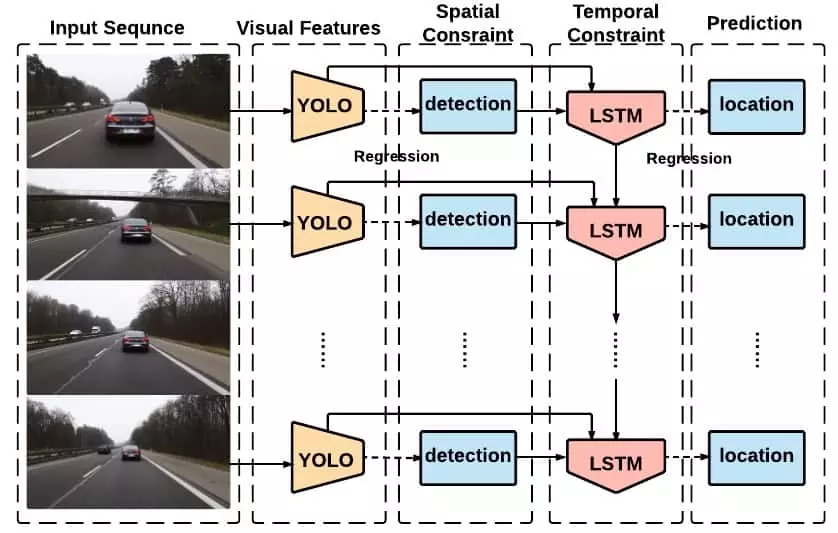
\includegraphics[width=1\textwidth]{rolo.png}
  \caption[Exemplo do funcionamento da arquitetura \ac{ROLO}]{
    \begin{itemize}
      \item \textbf{\ac{YOLO} INPUT}: Quadros de entrada brutos.
      \item \textbf{\ac{YOLO} OUTPUT}: Vetor de recursos de quadros de entrada e coordenadas da caixa delimitadora.
      \item \textbf{\ac{LSTM} INPUT}: Junção dos recursos da imagem e coordenadas da caixa delimitadora.
      \item \textbf{\ac{LSTM} OUTPUT}: Coordenadas da caixa delimitadora do objeto a ser rastreado.
    \end{itemize}
  }
\end{figure}

O diagrama \ref{img:rolo} fornece-nos o seguinte entendimento.
Os quadros de entrada passam pela rede \ac{YOLO}. Nesta rede, são obtidas duas saídas diferentes (Recursos de imagem e coordenadas da caixa delimitadora). Estas duas saídas são fornecidas à rede \ac{LSTM}. O \ac{LSTM} gera trajetórias, isto é, a caixa delimitadora do objeto a ser rastreado. A inferência preliminar de localização (do \ac{YOLO}) ajuda o \ac{LSTM} a prestar atenção a certos  elementos visuais. O \ac{ROLO} explora a história espaço-temporal, ou seja, juntamente com o histórico de localização, o \ac{ROLO} também explora a história dos recursos visuais. Mesmo quando a deteção do \ac{YOLO} falha devido a desfoque de movimento, o rastreamento de \ac{ROLO} permanece estável.


\subsection{KCF}
\label{chap2:subsec:rolo}

A ideia básica do \textbf{\ac{KCF}} é estimar um filtro de imagem ideal, de modo a que a filtragem com a imagem de entrada produza a resposta desejada.
Dado um conjunto inicial de pontos, o \ac{KCF} tenta calcular o movimento destes pontos observando a direcção da mudança no próximo quadro. Por isso este é um rastreador offline, que apenas funciona em vídeos gravados. Em cada quadro consecutivo, tentamos procurar o mesmo conjunto de pontos na vizinhança. Depois que as novas posições desses pontos são identificadas, podemos mover a caixa delimitadora sobre o novo conjunto de pontos. Há matemática envolvida para tornar a pesquisa mais rápida e eficiente.

\subsection{Centroid}
\label{chap2:subsec:centroid}

\paragraph{}
O \textbf{rastreamento de centroides} é um algoritmo presente na biblioteca \ac{OpenCV}, que depende da distância euclidiana\footnote{Distância entre dois pontos} entre centroides de objetos (objetos que o rastreador de centroide já viu antes) e novos centroides de objetos entre quadros subsequentes em um vídeo.
Neste algoritmo temos de usar um detector de objetos em cada quadro de vídeo e determinar os centroides de cada objeto. Assumimos aqui que no próximo quadro o centroide do objeto estará a uma curta distância no centroide no quadro anterior, e assim assumimos que seja o mesmo objeto através da distância. Este algoritmo não é muito eficiente em ambientes com mais que um objeto.

% https://cv-tricks.com/object-tracking/quick-guide-mdnet-goturn-rolo/
% https://missinglink.ai/guides/computer-vision/object-tracking-deep-learning/
% https://www.oreilly.com/library/view/computer-vision-with/9781788299763/0fbcf5be-a823-485e-a56e-454282e0d50d.xhtml

% Não incluido http://www.robots.ox.ac.uk/~joao/circulant/ mas bom em KCF

% https://www.pyimagesearch.com/2018/07/23/simple-object-tracking-with-opencv/



\section{Conclusões}
\label{chap2:sec:concs}

Neste capitulo foram descritos alguns dos algoritmos de deteção e rastreamento mais populares e eficientes. Podemos concluir que apesar da deteção e rastreamento de objetos ser uma ser ainda uma temática bastante recente teve já um grande avanço. Apesar da sua dificuldade e do seu nível computacional, cada vez existem mais algoritmos para melhorarem e tornarem o reconhecimento e rastreamento de objetos mais preciso e rápido.
\newline
Existem inúmeros algoritmos de detectores de objetos em imagens e de rastreadores de objetos em imagem. Em este capitulo foquei me em alguns dos mais populares e eficientes. Estes possuem na maioria versões mais leves em termos de peso computacional deles mesmos, versões que terei um especial foco no futuro devido ao ambiente de desenvolvimento, que é um Raspberry Pi. Foquei-me também em versões mais atuais, sendo a maioria baseadas em Aprendizagem Profunda e Redes Neurais.


% Falar de Tensorflow, Opencv ?
% Mais métodos ?? https://medium.com/@manivannan_data/multiple-object-tracking-algorithms-a01973272e52


\clearpage{\thispagestyle{empty}\cleardoublepage}
\chapter{Tecnologias e Ferramentas Utilizadas}
% OU \chapter{Trabalhos Relacionados}
% OU \chapter{Engenharia de Software}
% OU \chapter{Tecnologias e Ferramentas Utilizadas}
\label{chap:tecno-ferra}

\section{Introdução}
\label{chap3:sec:intro}
Cada capítulo \underline{intermédio} deve começar com uma breve introdução onde é explicado com um pouco mais de detalhe qual é o tema deste capítulo, e como é que se encontra organizado (i.e., o que é que cada secção seguinte discute).

\section{Secções Intermédias}
\label{chap3:sec:...}

A tabela~\ref{tab:exemplo} serve apenas o propósito da exemplificação de como se fazem tabelas em \LaTeX.
%
\begin{table}
\centering
\begin{tabular}{|c|lr|}
\hline
\textbf{campo 1} & \textbf{campo 2} & \textbf{campo 3}\\
\hline
\hline
14 & 15 & 16 \\
\hline	
13 & 13 & 13 \\
\hline
\end{tabular}
\caption{Esta é uma tabela de exemplo.}
\label{tab:exemplo}
\end{table}

\section{Conclusões}
\label{chap3:sec:concs}
Cada capítulo \underline{intermédio} deve referir o que demais importante se conclui desta parte do trabalho, de modo a fornecer a motivação para o capítulo ou passos seguintes.
\clearpage{\thispagestyle{empty}\cleardoublepage}
\chapter{Implementação e Testes}
% Os titulos dados aos capítulos são meros exemplos. Cada relatório deve adequar-se ao projeto desenvolvido.
\label{chap:imp-test}

\section{Introdução}
\label{chap4:sec:intro}
Cada capítulo \underline{intermédio} deve começar com uma breve introdução onde é explicado com um pouco mais de detalhe qual é o tema deste capítulo, e como é que se encontra organizado (i.e., o que é que cada secção seguinte discute).

\section{Secções Intermédias}
\label{chap4:sec:...}

O trecho de código seguinte mostra a função \texttt{main()} e o seu funcionamento:
\begin{lstlisting}[caption=Trecho de código usado no projeto.]
#include <stdio.h>

int main(){
  int i = 0;
  for(i = 0; i < 100; i++)
    printf("%d\n",i);
}
\end{lstlisting}


Se quiser definir a distribuição de Pareto, posso colocar a fórmula \emph{inline}, da seguinte forma $P(x)=\frac{x^{1/\Lambda}_{i}}{2}$, ou numa linha em separada, como se mostra a seguir:
$$ y^2 = \sum_{x=0}^{20}( x^3 - 2x + 3).$$

Outra maneira, mas numerada, é usar o ambiente \texttt{equation}, como se mostra na (\ref{eq:eq1}):
\begin{equation}
 y^2 = \sum_{x=0}^{20}( x^3 - 2x + 3).
 \label{eq:eq1}
\end{equation}

\begin{align}
 2+2+2+2+2+2+2+2+2+2+y^2 = & \sum_{x=0}^{20}( x^3 - 2x + 3);\\
                         = & x^4 -2.
 \label{eq:eq2}
\end{align}


\section{Conclusões}
\label{chap4:sec:concs}
Cada capítulo \underline{intermédio} deve referir o que demais importante se conclui desta parte do trabalho, de modo a fornecer a motivação para o capítulo ou passos seguintes.
\clearpage{\thispagestyle{empty}\cleardoublepage}
\chapter{Conclusões e Trabalho Futuro}
\label{chap:conc-trab-futuro}

\section{Conclusões Principais}
\label{sec:conc-princ}

Esta secção contém a resposta à questão: \\
\emph{Quais foram as conclusões princípais a que o(a) aluno(a) chegou no fim deste trabalho?}

\section{Trabalho Futuro}
\label{sec:trab-futuro}

Esta secção responde a questões como:\\
\emph{O que é que ficou por fazer, e porque?}\\
\emph{O que é que seria interessante fazer, mas não foi feito por não ser exatamente o objetivo deste trabalho?}\\
\emph{Em que outros casos ou situações ou cenários -- que não foram estudados no contexto deste projeto por não ser seu objetivo -- é que o trabalho aqui descrito pode ter aplicações interessantes e porque?}
\clearpage{\thispagestyle{empty}\cleardoublepage}

% SE EXISTIREM APENDICES, DESCOMENTAR O QUE ESTÁ EM BAIXO
% \appendix
% \include{apendice1}
% \clearpage{\pagestyle{empty}\cleardoublepage}
% \include{continuacao}
% \clearpage{\pagestyle{empty}\cleardoublepage}
% \include{apendice2}
% \clearpage{\pagestyle{empty}\cleardoublepage}
% \include{apendice3}
% \clearpage{\pagestyle{empty}\cleardoublepage}

\backmatter

\bibliographystyle{plain}
\bibliography{bibliografia}

\end{document}